\section{Solución implementada}

Se realizó la implementación de tres casos de uso sobre los distintos ecosistemas a analizar. Presentamos un análisis cualitativo y cuantitativo de las ventajas y desventajas de cada caso.

A continuación se detalla en qué consiste cada caso de uso.

\subsection{Casos de uso}

\subsubsection{Sitio web informativo}

Este es el caso más simple, donde no se requiere ningún tipo de procesamiento. El contenido que tiene este sitio es información sobre los casos de uso implementados, como también instrucciones o referencias de sus ecosistemas de despliegue.

\paragraph{Requisitos funcionales}

\begin{itemize}
    \item \textbf{Landing page del proyecto}: sitio web informativo donde se presente lo que se fue haciendo en este proyecto, información sobre los casos de uso y sus ecosistemas de despliegue.
\end{itemize}

\subsubsection{Repositorio de conocimiento}

Con este caso estaríamos analizando la capacidad de creación y modificación de contenido existente. La idea es que sea un servicio comunitario donde agregar información de distinta índole, similar a Wikipedia. Se podrán crear usuarios con roles de moderador y editor. Los moderadores tendrán mayor poder de decisión sobre qué contenido publicar y qué no, además de poder bloquear usuarios de ser necesario. Los editores se encargarán de agregar, eliminar y modificar el contenido del sitio buscando tener la información lo más actualizada posible. Este servicio contará con un front end, back end y una base de datos distribuidas utilizando la tecnología OrbitDB.

\paragraph{Requisitos funcionales}

\begin{itemize}
    \item \textbf{Edición:} los artículos dentro del repositorio deben ser editables por cualquier persona que ingrese al sitio, y este cambio debe verse reflejado (eventualmente) en las demás personas que accedan a ese artículo.
    \item \textbf{Historial de versiones:} cada artículo debe tener una lista de versiones anteriores, junto con hipervínculos con los cuáles acceder a ellas (mientras estén disponibles en la red).
    \item \textbf{Búsqueda:} una persona debe poder realizar una búsqueda global de todos los artículos.
\end{itemize}

\subsubsection{Mensajero en tiempo real}

Este caso se enfoca en la capacidad de la infraestructura de enfrentarse a situaciones de \textit{tiempo real} como puede ser un chat de texto o de audio. En particular nos centraremos en el caso de chats de texto para un grupo de usuarios en donde los mensajes sean públicos. Este servicio también contará con front end, back end y una base de datos donde persistir los mensajes.

\paragraph{Requisitos funcionales}

\begin{itemize}
    \item \textbf{Usuarios:} se deben contar con usuarios que puedan iniciar sesión con una contraseña.
    \item \textbf{Grupos públicos:} grupos de chat de texto, donde cualquier usuario puede ingresar y ver los mensajes del resto, así como también participar enviando sus propios mensajes.
\end{itemize}

\subsection{Proceso de descubrimiento}

Durante la implementación de los casos de uso para cada ecosistema, se fue desarrollando un mejor entendimiento de lo que se estaba creando. Logrando así generar distintas abstracciones que representan la infraestructura general para la implementación de los casos de uso.

Para cada ecosistema hay 2 principales infraestructuras en acción. La infraestructura de despliegue y la infraestructura de aplicación.

La \textbf{infraestructura de despliegue} es la encargada del "hosting" de una aplicación web. Con esta se distribuye y permite el acceso a lo que es el "front end" de las aplicaciones, como también el código para el funcionamiento de la aplicación, si se trata de una aplicación no estática. Cualquier aplicación que desee ser accedida por la web va a hacer uso de esta infraestructura, como es el caso del sitio web informativo.

La \textbf{infraestructura de aplicación} es la encargada de la lógica de la aplicación, como es el almacenamiento de datos. Aplicaciones que requieran de mantener un estado y permitir la modificación de parte de los usuarios van a necesitar hacer uso de esta infraestructura, como es el caso del repositorio de conocimiento y mensajero en tiempo real.

(Mover a IPFS esto, ya que no se hicieron abstracciones en blockchain) Al lograr encontrar estas abstracciones, se permite que generar nuevos casos de uso sea mucho más fácil, ya que la mayoría de la lógica sobre el el ecosistema se encuentra encapsulada dentro de ellas, logrando que el desarrollo de un nuevo caso de uso se concentre únicamente en sus requisitos y no en el ecosistema en el que se encuentra.

A continuación se va a explicar como se componen y funcionan ambas infraestructuras en cada ecosistema.

(Explicar que lo que hicimos son packages)

\subsection{IPFS}

\subsubsection{Infraestructura de despliegue}

En IPFS, es posible desplegar una aplicación web subiendo un directorio con todos los archivos estáticos necesarios para el funcionamiento en un navegador, incluyendo el código necesario a nivel aplicación. Esto se puede realizar manualmente mediante cualquier cliente de IPFS, como \cite{kubo} o \cite{helia}, y devuelve un \textit{Content identifier} (CID) \cite{cid} que representa esa versión de la aplicación.

Las aplicaciones web son una de los principales casos de uso de IPFS. Los sitios web estáticos se complementan con el \textit{content addressing}, ya que su CID se mantiene y no requiere cambiar hasta que se actualice su contenido. Cualquier usuario puede publicar su sitio web en la red de IPFS a través de un nodo local de manera gratuita y poco tiempo. IPFS provee un tutorial en su página de cómo realizarlo \cite{ipfs-static-website}. A continuación se detallará las implicaciones que tiene desplegar una aplicación web de esta manera, y que alternativas existen para publicar en IPFS.

Al subir un archivo, por ejemplo código HTML, este se transforma en una representación de contenido direccionable mediante un CID. Desde ese momento, cualquier nodo que quisiese obtener el archivo, puede encontrarlo mediante su CID. Sin embargo, no se asegura la persistencia del archivo, y dejará de ser accesible luego de un tiempo. Se debe al \cite{garbage-collector} implementado por IPFS, que desecha datos para liberar almacenamiento de forma arbitraria. Es por esto que existe el concepto de \cite{pinning}: \textit{"pinear"} un archivo significa instruir al nodo IPFS para tratar a un archivo o directorio presente en la red de IPFS como esencial y, por lo tanto, no descartarlo. Sin embargo, \textit{"pinear"} el archivo o directorio, no significa que estará disponible de forma indeterminada en el tiempo, debido a que todavía depende de que el nodo que esté pineando el contenido esté activo, o que otros nodos que hayan accedido al archivo aún lo tengan en su caché para permitir que otros puedan acceder a él. Además, para mejorar la disponibilidad de un archivo, el caso ideal sería que varios nodos "pineen" el archivo, de manera que otros nodos que quieran obtener el contenido puedan hacerlo desde cualquiera de estos nodos.

Para lograr que el contenido persista en la red sin necesidad de que el nodo local esté activo, existen opciones para delegar el \textbf{pineo} del archivo o directorio. Existen servicios de \textit{pinning} y clusters colaborativos, que actuan pinneando los archivos en múltiples nodos, aumentando no solo su disponibilidad sino también su distribución, y por ende logrando un acceso más rápido al contenido.

\paragraph{Servicios de \textit{pinning}}

La manera más fácil de asegurarse que los datos estén disponibles y se persistan es usar un servicio de \textit{pinning} \cite{pinning-services}. Estos servicios cuentan con varios nodos que pinnean archivos. De esta manera, ya no es necesario contar con un nodo local que los aloje. Algunos ejemplos de servicios de pinning incluyen Fleek \cite{fleek} y Pinata \cite{pinata}.

Desde el punto de vista de las aplicaciones estrictamente comunitarias, estos servicios no van de la mano con su filosofía. Por un lado, los servicios de \textit{pinning} tienen un modelo gratis con funcionalidad limitada o capacidad de almacenamiento limitado. Por otro lado, se depende de estos servicios, lo que en esencia centraliza el proceso de despliegue de la aplicación o sitio web. Si por algún motivo el servicio dejara de "pinear" los archivos, estos pueden dejar de estar disponibles en la red IPFS, e incluso pueden perderse por completo. Esto rompe completamente con la naturaleza de aplicaciones descentralizadas y pasa a tener una centralización tercerizada similar a utilizar AWS.

\paragraph{Clusters colaborativos}

Estos son grupos de nodos de IPFS que actuan colaborativamente para "pinear" el contenido que se agregue al cluster, por uno o múltiples peers. De esta manera, podemos lograr que los usuarios opten por colaborar con su nodo local para el "pinneo" de la aplicación. Así, se logra que la misma comunidad mantenga en servicio el mecanismo de despliegue de la aplicación, lo cuál es acorde a la filosofía de aplicaciones comunitarias.

Actualmente, esta alternativa es que es poco explorada, por lo tanto no existe una forma fácil de creación, seguimiento y descubrimiento de estos clusters. IPFS cuenta con una página con clusters conocidos con los cuales se puede colaborar, pero la cantidad de clusters es limitada.

Por otro lado, el principal problema es que los clusters obligan a los nodos a "pinear" la totalidad de sus archivos, lo cuál puede significar el uso de cientos de gigabytes en almacenamiento necesarios únicamente para colaborar. Pinear parte del contenido es imposible actualmente. Esto se debe a que, debido a la manera en la que fue diseñada la arquitectura de IPFS, un nodo puede mentir acerca de los archivos que tiene, por lo que hay una posibilidad de que una parte del contenido no esté en ninguno de los nodos, y por ende el contenido esté incompleto.

\paragraph{Acceso y mutabilidad}

Para buscar un contenido, un nodo de IPFS realiza una búsqueda a través de su CID, el cual es único. Debido a que es único, el CID cambiará si el contenido del sitio web o aplicación web cambia, ya que el contenido será distinto. Esto vuelve el proceso de despliegue altamente impráctico, ya que se necesitaría compartir un nuevo CID cada vez que se actualice una página.

Este problema puede ser resuelto con la ayuda de \textit{punteros mutables}. Estos punteros son un objeto de IPFS que apunta a un CID determinado, previamente elegido por el usuario. El CID al que apunta el puntero puede ser cambiado, por lo tanto permiten compartir la dirección del puntero una única vez y actualizar el CID al cuál apunta cada vez que se haga un cambio.

\subparagraph{IPNS}

El InterPlanetary Name System (IPNS) \cite{ipns} es un sistema que permite crear  punteros mutables y obtener su dirección en forma de CIDs conocidos como \textit{names} o \textit{nombres de IPNS}. Estos nombres de IPNS pueden considerarse como enlaces que pueden actualizarse, conservando al mismo tiempo la verificabilidad del content addressing.

Un nombre de IPNS es un hash de una clave pública. Está asociado a un \textit{IPNS record} que contiene la ruta a la que se vincula, entre otra información. El titular de la clave privada puede firmar y publicar nuevos registros en cualquier momento.

*Gráfico de IPNS*

Es posible utilizar IPNS con uno de estos posibles enfoques:
\begin{itemize}
    \item \textbf{Consistencia:} garantizar que los usuarios siempre resuelvan el último registro de IPNS publicado, a riesgo de no poder resolverlo.
    \item \textbf{Disponibilidad:} resolver un registro de IPNS válido, a costa de potencialmente resolver un registro desactualizado -o sea, con un CID previo.
\end{itemize}

El registro IPNS se encuentra a través de la \textbf{Distributed Hash Table} (DHT). Todos los nodos de IPFS participan alojando colaborativamente el contenido de la DHT. Por lo tanto, el DHT actúa como un "directorio" descentralizado, donde la clave pública es un identificador. Esta tabla ayuda a localizar el registro IPNS que apunta al contenido deseado, entre otras funciones. Para entender mejor cómo IPNS funciona se puede consultar la documentación de IPFS.

IPNS es una buena forma de obtener mutabilidad dentro de IPFS. Una vez que se aloja un contenido en IPFS y se apunta a él mediante un \textit{IPFS name}, el mayor problema pasa a ser la manera de acceder a IPNS en sí. El hecho de que los names sean hashes alfanuméricos, y no nombres legibles o memorables para humanos, representa una dificultad adicional a la hora de alojar un sitio web al cuál los usuarios puedan acceder fácilmente. A continuación se analizará dos alternativas para solucionar este problema.

(explicar como se puede utilizar con un cluster colaborativo a traves de pub sub)

\subparagraph{DNSLink}

IPNS no es la única forma de crear mutable pointers en IPFS. DNSLink \cite{dnslink} utiliza registros \textit{DNS TXT} para asignar un nombre DNS (por ejemplo, un dominio) a una dirección IPFS o a un \textit{IPNS name}. Como uno puede editar sus registros DNS, puede usarlos para que siempre apunten a la última versión de un objeto en IPFS.

DNSLink actualmente es mucho más rápido que IPNS, utiliza nombres legibles por humanos y también puede apuntar a nombres IPNS. A pesar de ello, tiene un problema muy fundamental y es que se utiliza el protocolo DNS, el cual tiene claras deficiencias con la filosofía de aplicaciones comunitarias.

La más importante es que, aunque DNS tenga claras ventajas, como que es un sistema distribuído y escalable, es también un sistema algo centralizado. Las autoridades centrales como \textit{ICANN} gestionan las raíces del DNS. Esto hace que un registro DNS sea fácil de censurar, a nivel de registrador como también de los \textit{ISPs}.

\subparagraph{ENS}

ENS, Ethereum Name Service es el protocolo de nombres descentralizado que se basa en la Ethereum blockchain. Funciona de manera similar a DNS, en el sentido de que los nombres ENS resuelven a nombres legibles para humanos. Como esto se computa en la blockchain de Ethereum, es seguro, descentralizado y transparente.

Es posible configurar un registro ENS para que se resuelva en la dirección IPNS, proporcionando nombres legibles para humanos que son más fáciles de compartir y acceder, y solucionando el principal problema de IPNS hasta este punto.

Un registro de ENS puede apuntar a un \textit{IPNS name}, haciendo uso de las ventajas de ambos sistemas. Cuando se quiera actualizar el contenido, no será necesario modificar el registro ENS en sí, ya que siempre se va a apuntar al mismo name de IPNS.

Cabe aclarar que adquirir un dominio ENS tiene un costo, es un costo el cual no suele ser muy elevado y trae todos los beneficios mencionados, especialmente para sitios web estáticos y también cualquier aplicación comunitaria. Pero sigue siendo un paso opcional en el despliegue de sitios web o web apps, ya que el IPNS name sigue siendo completamente accesible sin un registro de ENS apuntanto a él.

\paragraph{Despliegue continuo}

En un proyecto de aplicación web centralizada, es común automatizar el proceso de despliegue con cada cambio que se realiza. Normalmente este proceso se activa con cada nuevo commit en una rama de Git especifica, e incluye todas las etapas necesarias para convertir el contenido de un repositorio Git en código estático listo para ser desplegado. También puede incluir más pasos que incluyan actualizaciones en el backend.

Yendo al caso específico de aplicaciones web comunitarias, el script debe ser ejecutado en los nodos confiables, ya que una \textit{Github action} no puede utilizar un nodo IPFS que requiera puertos abiertos. En este tipo de aplicaciones, al tener una jerarquía mayormente horizontal, no hay un servidor central que orqueste esta actualización, sino que se necesita que cualquier nodo confiable pueda actualizar su contenido e instruir a los nodos colaborativos para actualizar su contenido de igual forma. Todo esto debe ser posible incluso cuando los nodos no reciben la actualización al mismo tiempo, es decir, no debe haber \textit{race conditions}.

Una forma de lograr esto es, por ejemplo, utilizar un algoritmo de elección de líder u otro algoritmo distribuido para elegir el nodo responsable de indicar el nuevo contenido a pinear al resto de nodos en el cluster. Sin embargo, esta manera de realizar la actualización implica una capa adicional de complejidad que no es necesaria debido a la naturaleza de IPFS.

Como ya se ha mencionado, si dos nodos suben el mismo contenido, obtendrán el mismo CID. Esto puede ser utilizado para que cualquier nodo confiable pueda actualizar el contenido y el nombre de IPNS independientemente del resto de los nodos confiables. Cuando se detecte un cambio nuevo, el nodo puede obtener el código estático, y acto posterior, indicar al resto de los nodos del cluster que pineen el CID especifico. En el caso de que sea el primer nodo en detectar el cambio, deberá instruir al resto del cluster para que dejen de pinear el CID antiguo. En el caso en que otro nodo haya detectado la actualización antes, no deberá actualizar ningún pin del cluster debido a que el mismo CID ya va a estar presente en la lista de pins.

\paragraph{Compilación} Las herramientas de compilado no siempre son deterministas en los archivos compilados que genera. Next.js, por ejemplo, genera diferentes archivos estáticos en dos compilaciones basadas en el mismo código fuente. Esto es un problema para el enfoque propuesto, debido a que si dos nodos compilan el mismo código, el CID puede ser diferente. Para mitigar esto, se decidió hacer uso de un \textit{hook} que compile el código con cada \textit{commit} en la rama principal una única vez por cambio realizado. De esta manera, los nodos confiables pueden detectar el cambio en la rama utilizada para alojar los archivos estáticos, y hacer \textit{pull} sobre esos archivos y, por lo tanto, obtener un mismo CID.

\paragraph{service.json} Para que un usuario pueda conectarse y contribuir como colaborador a un cluster, la herramienta de terminal \textit{\textbf{ipfs-cluster-follow}} requiere una dirección de IPFS de la cuál obtener el archivo \textit{service.json}. Este archivo de configuración contiene todos los datos necesarios para que un colaborador pueda unirse. Además, está sujeto a modificaciones, debido a que el archivo contiene las \textit{multiaddresses} de cada nodo confiable en forma de lista, por lo que agregar o remover un nodo confiable implica modificar el archivo.

Es por esto que el proceso de despliegue también debe incluir este archivo. Debe incluirse la detección de una actualización, el pineo del nuevo \textit{service.json} al cluster, 

\paragraph{Enfoque}

En base a este análisis, podemos concluir que la mejor forma de desplegar una página web estática en IPFS es a través del uso de un cluster colaborativo compuesto por nodos confiables y nodos colaboradores, así como una dirección IPNS a la cuál actualizar cada vez que hay un cambio, y un registro ENS para traducir la dirección IPNS a un nombre legible.

Este enfoque tiene, sin embargo, desventajas o aspectos a mejorar:

\subparagraph{Necesidad de tener nodos confiables} Estos nodos van a ser los encargados de administrar el cluster, y actualizar el IPNS. La distinción entre nodos confiables y nodos colaborativos es necesaria para evitar que un potencial atacante pueda modificar el CID al que apunta el \textit{IPNS name} o modificar el contenido que pinea el cluster colaborativo.
 
\subparagraph{Actualización del contenido} Por cada cambio que se realice en el directorio de la página, se deberá pinear el nuevo contenido al cluster, y por lo tanto todos los colaboradores tendrán que obtener todo el directorio nuevamente. Esto puede claramente volverse costoso con contenido de tamaño considerable.
    
\subparagraph{Cache de IPNS} El parámetro TTL de IPNS indica cuanto "vive" un valor asociado a un nombre de IPNS en la cache de un nodo antes de forzar a este a volver a buscar el valor en la DHT. El problema que tiene esto es que, si se pone un valor muy elevado, un nodo gateway no buscará la actualización hasta que se cumpla el periodo y por lo tanto el registro de IPNS no se actualizará. Por otro lado, si se pone un valor muy corto, siempre se buscará el valor en la DHT, generando latencia al no utilizar el cache disponible. Pero a su vez, el nombre de IPNS en un nodo siempre tendrá la última versión que encuentre.

\subparagraph{Compartir claves privadas} Cómo la actualización de un nombre de IPNS está firmada con una clave privada, todos los nodos confiables deberan tener la misma clave para poder potencialmente actualizar el registro IPNS y así evitar tener un único nodo con esa responsabilidad. Esto elimina un punto de falla único, pero aumenta las chances de que esa clave privada llegue a manos de un posible atacante.

\subparagraph{Necesidad de re-publicar el nombre de IPNS cada cierto tiempo} Kubo (una de las implementaciones de un nodo de IPFS) actualiza el nombre de IPNS cada hora para asegurarse de que siga estando en la DHT. Pero si se cae el nodo que publicó último puede que no se actualice mas, esto se tiene que tener en cuenta

\subparagraph{Apertura de puertos} IPFS cluster utiliza el puerto 9096 para la comunicación entre nodos, el cual se tiene que abrir para un correcto funcionamiento. Se podría usar hole punching (?).

\subsubsection{Infraestructura de aplicación}

\subsection{Blockchain}

En este trabajo se utilizó la red de Ethereum, al ser una blockchain popular nos permite demostrar y comparar los casos de uso contra nuestra solución en IPFS. Ethereum está compuesta de nodos distribuidos que comparten poder de cómputo lo cual permite el desarrollo de aplicaciones descentralizadas. Cuenta con una moneda que funciona a modo de incentivo, es decir, que los nodos reciben ganancias por formar parte de la red. Esto conlleva a que los usuarios de la red necesiten pagar para utilizarla a través de transacciones.

\subsubsection{Swarm}

Para el desarrollo del sitio web estático se decidió ir por Swarm que es un almacenamiento descentralizado que corre sobre una \textit{sidechain} de Ethereum. Swarm surgió como uno de los tres pilares de Ethereum para una web descentralizada \parencite{swarm-origin}. Funciona por \textit{content addressing} como IPFS e incluye un modelo de incentivos utilizando su propia moneda llamada BZZ.

\paragraph{Feed}

Los \textit{feeds} en Swarm funcionan de manera similar a los IPNS de IPFS. Es un puntero, con CID fijo, a un archivo. Esto permite actualizar el archivo al que apunta un \textit{feed} manteniendo un punto de entrada fijo al sitio web.

\subsubsection{Ethereum}

Para los casos de uso del repositorio de conocimiento y el mensajero en tiempo real necesitamos una herramienta que nos funcione de manera \textit{read-write} y como Swarm solamente se encarga de archivos estáticos buscamos alguna alternativa dentro del ecosistema blockchain. Para esto terminamos usando Ethereum.

\begin{figure}[H]
    \centering
    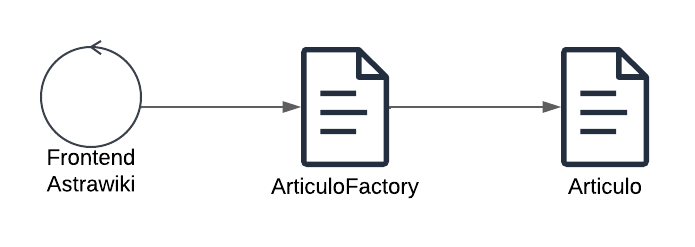
\includegraphics[width=0.5\linewidth]{img/astrawiki-articulo-factory.png}
    \caption{\textit{Smart contracts} que intervienen en el repositorio de conocimiento}
    \label{fig:aw-eth-articulo-factory}
\end{figure}

Ambos casos de uso resultaron muy similares en su resolución, haciendo uso del patrón de diseño \textit{Factory}. Existe un smart contract Factory que crea otros smart contracts (Artículo o Chat, según el caso de uso).

\begin{figure}[H]
    \centering
    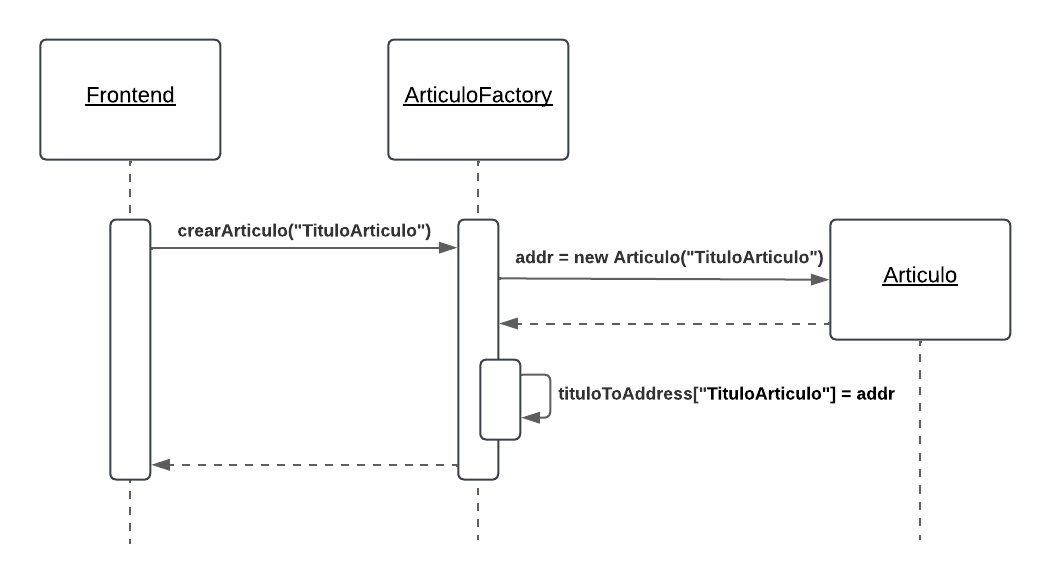
\includegraphics[width=0.75\linewidth]{img/ds-aw-eth-crear-articulo.png}
    \caption{Creación de un artículo}
    \label{fig:ds-aw-eth-crear-articulo}
\end{figure}

De esta manera el \textit{Factory} tiene un \textit{mapping} con todos los artículos creados y las direcciones correspondientes para accederlos. Si se quisiera acceder a un Artículo en particular primero se tiene que consultar al \textit{Factory} para obtener la dirección del mismo y, como cada artículo es un \textit{smart contract} en sí mismo, se puede consultar o modificar su contenido directamente interactuando con el Artículo en particular como se puede ver en la Figura \ref{fig:ds-aw-eth-obtener-contenido-articulo}.

\begin{figure}[H]
    \centering
    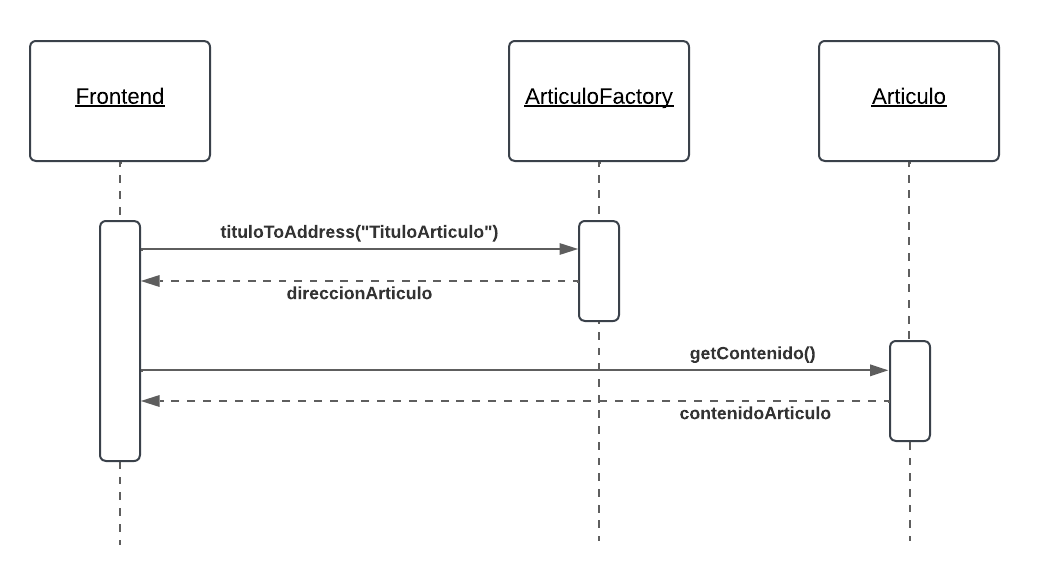
\includegraphics[width=0.75\linewidth]{img/ds-aw-eth-obtener-contenido-articulo.png}
    \caption{Obtención del contenido de un artículo}
    \label{fig:ds-aw-eth-obtener-contenido-articulo}
\end{figure}

La principal diferencia entre el repositorio de conocimiento y el mensajero en tiempo real está en que los mensajes del mensajero tienen que ser vistos por los demás usuarios que participan de la conversación en el momento que se envían. Esto no es estrictamente necesario en el repositorio de conocimiento pero sí lo es en el mensajero.

Para afrontar este requisito se utilizaron los eventos de Solidity (el lenguaje de programación en el que se desarrollan los \textit{smart contract} de Ethereum). Funciona de la siguiente manera, al momento de enviar un mensaje se emite un evento. Este evento se recibe en un listener que fue previamente inicializado al instante previo de haber obtenido el Chat en el frontend. Al recibir este evento el frontend puede actualizar la pantalla mostrando el mensaje nuevo sin necesidad de obtener todos los mensajes.

% TODO: insertar gráfico del flujo de un evento al enviar un mensaje 

Por otro lado, para el mensajero en tiempo real necesitamos una manera de identificar a cada usuario. Para esto se hizo uso de las \textit{wallets}. Cada usuario se identifica utilizando su \textit{wallet}, que tiene una clave pública, que pasa a ser el identificador del usuario, y una clave privada la cuál es necesaria para firmar transacciones en nombre del usuario, que en nuestro caso funciona a modo de contraseña. Además, para que la lectura de las conversaciones sean más usables, se agregó la posibilidad de generar un nombre de usuario asociado al identificador del mismo. A este nombre de usuario lo llamamos alias y es único para todos los Chats asociados a un mismo ChatFactory. Una vez el usuario se conecta con su \textit{wallet}, puede elegir un alias y cambiarlo cuando desee siempre y cuando no exista actualmente algún otro usuario con ese mismo alias.

Finalmente, nos queda la funcionalidad de que un usuario pueda responder a otro mensaje. Primero necesitamos una manera de identificar a cada mensaje de manera unívoca. El identificador de cada mensaje se genera hasheando el timestamp del bloque, el identificador del emisor y la cantidad de mensajes en el chat en el momento que se envía. Luego, cuando se responde a otro mensaje se almacena el identificador del mensaje al que se está respondiendo (el mensaje padre) dentro de la estructura del mensaje que se está enviando. Todo esto se resuelve dentro del \textit{smart contract} del Chat correspondiente.


\subsection{FrontEnd}

Astraweb